% VUT FIT MITAI
% MSZ 2021/2022
% Author: Vladimir Dusek
% Login: xdusek27

%%%%%%%%%%%%%%%%%%%%%%%%%%%%%%%%%%%%%%%%%%%%%%%%%%%%%%%%%%%%%%%%%%%%%%%%%%%%%%%%

% Path to figures
\graphicspath{{avs/paralelni_zpracovani_v_openmp/figures}}

%%%%%%%%%%%%%%%%%%%%%%%%%%%%%%%%%%%%%%%%%%%%%%%%%%%%%%%%%%%%%%%%%%%%%%%%%%%%%%%%

\chapter{AVS~--~Paralelní zpracování v OpenMP: Smyčky, sekce a tasky a synchronizační prostředky.}

%%%%%%%%%%%%%%%%%%%%%%%%%%%%%%%%%%%%%%%%%%%%%%%%%%%%%%%%%%%%%%%%%%%%%%%%%%%%%%%%

\section{Zdroje}

\begin{compactitem}
    \item Moje materiály ke zkoušce z AVS.
    \item \path{AVS-07.pdf}
    \item \path{AVS-08.pdf}
    \item \path{AVS-10.pdf}
    \item \textit{Otázka není vysázená, pouze vloženo exportované PDF z google docs.}
\end{compactitem}

%%%%%%%%%%%%%%%%%%%%%%%%%%%%%%%%%%%%%%%%%%%%%%%%%%%%%%%%%%%%%%%%%%%%%%%%%%%%%%%%

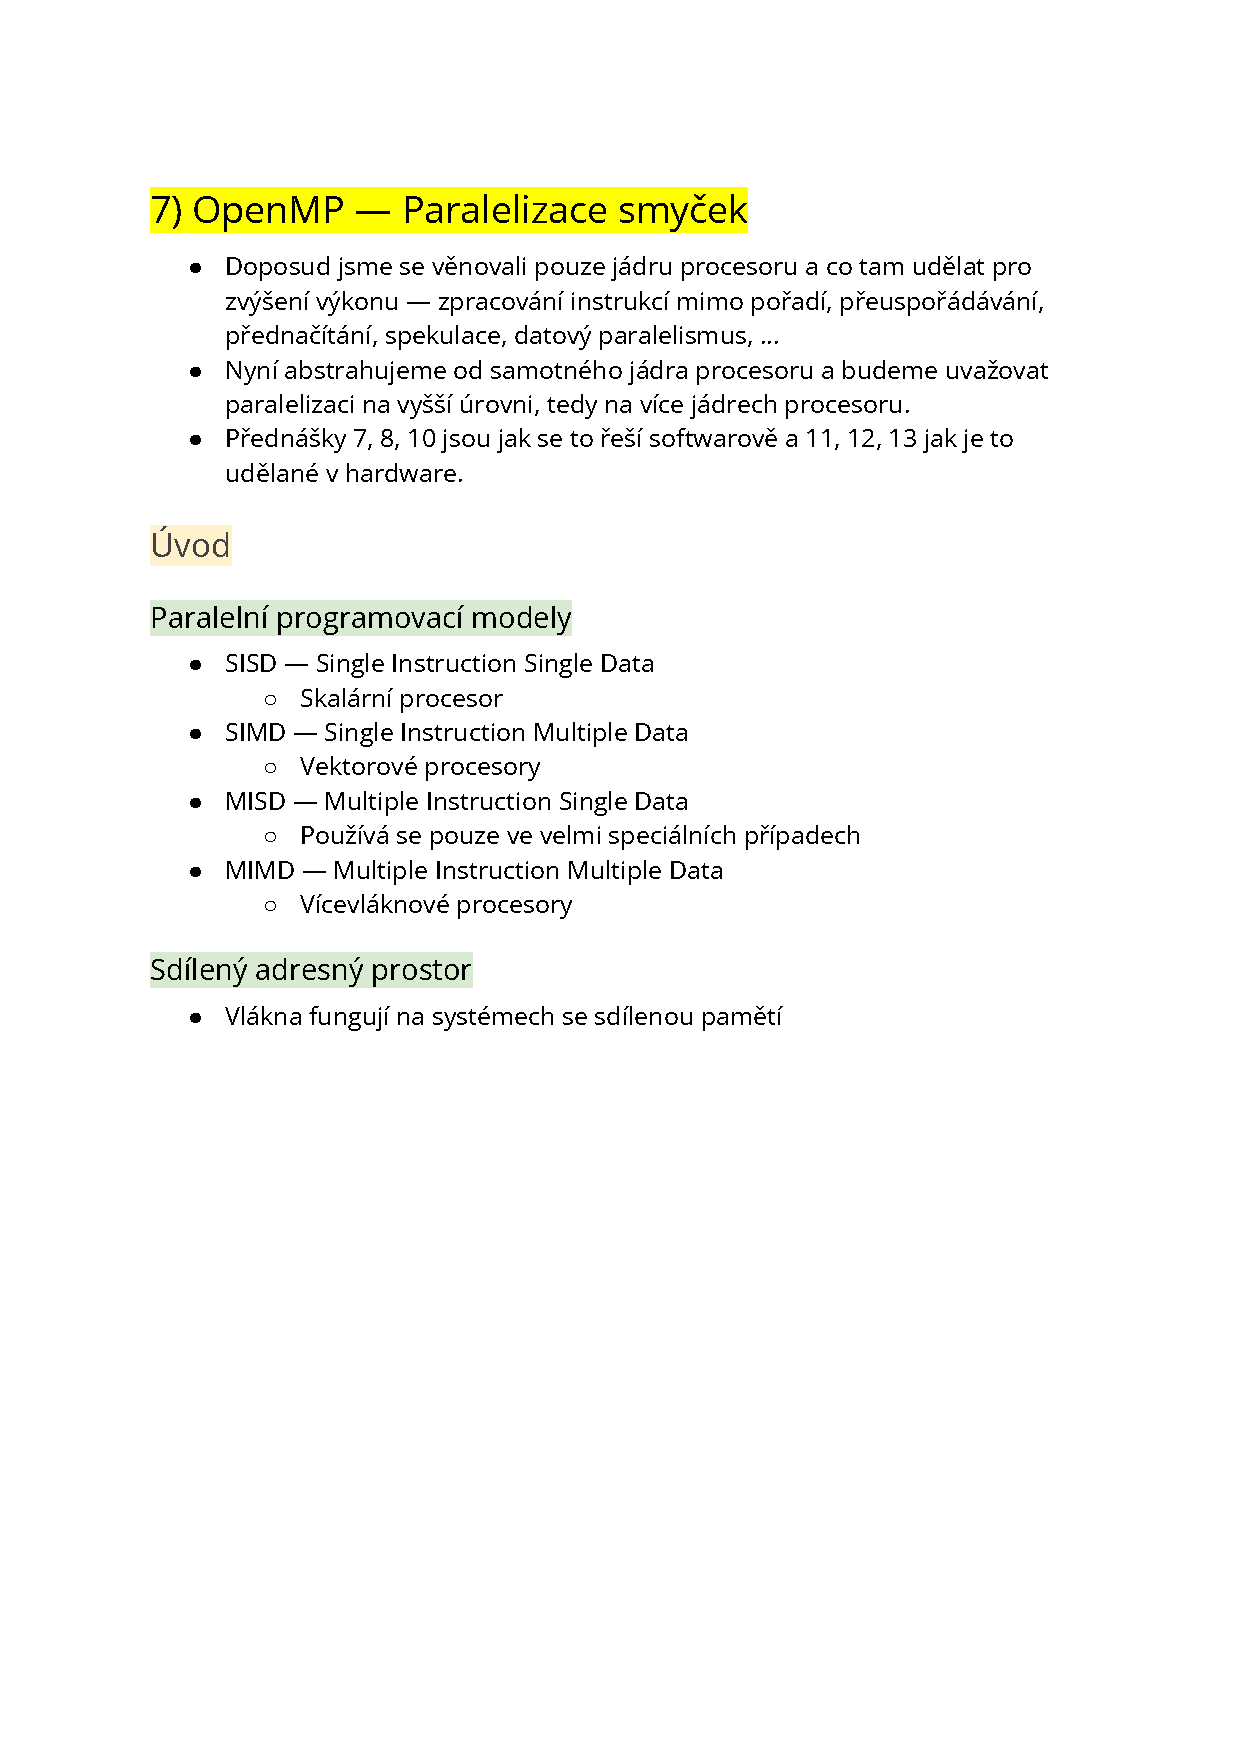
\includepdf[pages=-]{avs/paralelni_zpracovani_v_openmp/gdocs-avs-openmp.pdf}

% \section{Úvod a kontext}

% \begin{compactitem}
%     \item Doposud jsme se věnovali pouze jak zvýšit výkon v rámci jednoho jádra procesoru -- zpracování instrukcí mimo pořadí, přeuspořádávání, přednačítání, spekulace, datový paralelismus, \ldots

%     \item Nyní abstrahujeme od samotného jádra procesoru a budeme uvažovat paralelizaci na vyšší úrovni, tedy na více jádrech procesoru. \begin{compactitem}
%         \item Přednášky 7, 8, 10 vysvětlují, jak se to řeší softwarově a 11, 12, 13 jak je to udělané v hardware.
%     \end{compactitem}

%     \item \textbf{Sdílený adresný prostor} \begin{compactitem}
%         \item Vlákna fungují na systémech se sdílenou pamětí.
%         \item Každé vlákno má svůj zásobník, tedy cokoliv naalokované staticky, je privátní pro vlákno.
%         \item Halda je společná pro všechna vlákna, tedy cokoliv naalokované dynamicky (malloc, new, \ldots) je sdílené.

%         \begin{figure}[H]
%             \centering
%             \includegraphics[width=0.9\linewidth]{sdileny_adresny_prostor.png}
%             \caption{Paměťový prostor a paralelizace na úrovni vláken.}
%         \end{figure}
%     \end{compactitem}

%     \item \textbf{Jak paralelizovat} \begin{compactitem}
%         \item Sekvenční jazyk + příkazy paralelního zpracování, komunikace a synchronizace.
%         \item Sekvenční jazyk + dynamické knihovny.
%         \item Sekvenční jazyk + direktivy pro kompilátor (pragma).
%         \item OpenMP API -- kombinace direktiv a knihovních programů.
%     \end{compactitem}

%     \item \textbf{Výpočetní model vláken} \begin{compactitem}
%         \item Vlákna jsou ovládaná a použitá kernelem OS.
%         \item Hardware vlákno.
%     \end{compactitem}

%     \item \textbf{Model zpracování vláken} \begin{compactitem}
%         \item Strukturovaný blok.
%         \item Na konci bloku bariéra -- sloučení vláken (zabití potomků).

%         \begin{figure}[H]
%             \centering
%             \includegraphics[width=0.9\linewidth]{parallel_regions.png}
%             \caption{Model zpracování vláken v rámci běhu programu.}
%         \end{figure}
%     \end{compactitem}
% \end{compactitem}

% %%%%%%%%%%%%%%%%%%%%%%%%%%%%%%%%%%%%%%%%%%%%%%%%%%%%%%%%%%%%%%%%%%%%%%%%%%%%%%%%

% \section{Vytvoření týmu vláken}

% \begin{compactitem}
%     \item \textbf{Direktiva}
%     \item \textbf{Dovětek} -- Upravuje chování direktivy.

%     \item Direktiva \texttt{pragma omp parallel} \begin{compactitem}
%         \item Vytvoření paralelních sekci (vlákna).
%     \end{compactitem}
% \end{compactitem}

% \noindent\begin{minipage}{\linewidth}
% \begin{lstlisting}[language=c_language, caption={Vytvoření paralelní sekce.}]
% omp_set_num_threads(4); // kolik ma mit sekce vlaken
% double a[1000];

% #pragma omp parallel [clause[clause]... ]
% {
%     int id = omp_get_thread_num(); // ziskej id vlakna
%     work(id, a);
% }
% \end{lstlisting}
% \end{minipage}

% \begin{compactitem}
%     \item Dovětek \texttt{private(list)} \begin{compactitem}
%         \item Udělat privátní kopii sdílené proměnné.
%         \item Deklaruje novou privátní proměnnou, ale neinicializuje.
%     \end{compactitem}
% \end{compactitem}

% \section{Paralelizace smyček}

% \todo{todo}

% Plánování iterací

% Paralelní sekce

% Tasky

% Vzájemné vyloučení

% Synchronizace událostmi

% Synchronizace programovaná uživatelem
